\begin{justify}
\chapter[Marco teórico]{Marco teórico}
\label{ch:marcoteorico}
En este capítulo se introducirán conceptos y problemas que serán abordados durante el desarrollo del proyecto, a través de la recopilación y análisis de información relacionada con el foco central de la investigación, además se explicará cada concepto clave relacionado al proyecto y luego se establecerá la relación de esta materia con el proyecto.

\section{ALOHAnet}
El sistema ALOHA, nació con el fin de crear un sistema que se adapte a aquellos escenarios donde las limitaciones de los diseños de redes computacionales implementados bajo conexiones cableadas no se adaptan a las condiciones a las que será expuesto, es decir, situaciones donde son preferibles las comunicaciones sobre la base de la radio frecuencia, por sobre las comunicaciones sobre las conexiones cableadas~\cite{NORMAN}.\\
La estructura de funcionamiento del sistema ALOHA, consta de un computador central conectado a un canal de comunicaciones por radio frecuencia, donde se poseerán dos bandas de un tamaño de \SI{100}{\kilo\hertz} en las bandas \SI{407.350}{\mega\hertz} y \SI{413.475}{\mega\hertz}, una de estas bandas estará destinada a la recepción de información desde los clientes al computador central, y la otra a el envío de información desde el computador central hacia los clientes, donde se genera un método de acceso aleatorio de multiplexación de un gran número de clientes de baja tasa de envío de datos hacia el computador central, donde la comunicación se lleva a cabo por un único canal de comunicaciones por radio~\cite{NORMAN}. Si bien los mensajes desde o hacia la computadora central no se pueden multiplexar, si se pueden utilizar técnicas como la multiplexación del canal y del tiempo, para dividir el canal de comunicaciones desde las consolas hacia la computadora central en un gran número de canales donde cada uno de los clientes usará una de estas subdivisiones del canal, esté activo o no, dado que si se otorgara tiempo de conexión exclusiva a una fracción del número total los clientes activos de la red, este esquema tendría las mismas deficiencias que el diseño de conexión cableada~\cite{Abdullah}.\\
Como puede apreciarse en la Fig~\ref{aloha:msg}, la estructura de los paquetes de datos que conformarán las trazas de datos en el protocolo ALOHA, constan de un tamaño de a lo más \SI{704}{\bit}, de los cuales pueden usarse \num{80} caracteres de \SI{8}{\bit} cada uno (un total máximo de \SI{640}{\bit} de \textit{payload}), \SI{32}{\bit} de control y paridad, más \SI{32}{\bit} de identificación. Estos paquetes están diseñados para transmitirse en un tiempo a lo más de \SI{29}{\milli\second} a una tasa de \SI{24000}{Bd} (número de símbolos/segundos)~\cite{NORMAN}.\\
\begin{figure}[!ht]
\centering
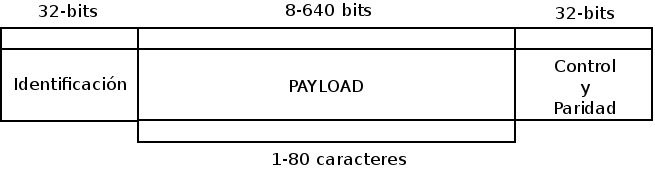
\includegraphics[scale=0.5]{images/alohamsg.png}
\caption{Formato de mensaje de protocolo ALOHA}
\label{aloha:msg}
\end{figure}\\
Con respecto al funcionamiento de este sistema ALOHA, este posee un tipo de conexión asíncrona donde los usuarios activos de una red con este sistema usarán un acceso aleatorio a la red, donde sólo se tomará en cuenta el tiempo donde se comienza el envío de los paquetes de datos y los canales disponibles para la transmisión (en base a la potencia del nodo y la disponibilidad del canal), dado que luego de esperar el doble del tiempo máximo de propagación, en el que  no recibe un paquete \gls{ack} que verifique la llegada del paquete enviado. El cliente retransmitirá este paquete periódicamente, hasta recibir un acuse de recibo por su contra parte. Para definir los límites de uso y capacidad del canal, se establece que el número máximo de clientes simultáneos en la red es de \num{324} clientes, dado que sobre dicho valor, la comunicación se vuelve inestable y con esto, el número promedio de retransmisiones se vuelve ilimitado por lo que satura el canal de comunicaciones~\cite{NORMAN}.\\
Este sistema es de vital importancia para este proyecto de título, dado que los dispositivos LoRa basan su comunicación en un sistema ALOHA puro (sistema descrito en esta sección), y ALOHA slotted o ``ALOHA \textit{con espacios}''. En la variante slotted del protocolo ALOHA, se agrega una comprobación de canal si está ocupado o no antes de transmitir, esta comprobación es llamada \gls{lbt}~\cite{Sornin}~\cite{Sornin2}. De esta manera se aumenta el \textit{throughput} por fracción de tiempo, por lo que es central el tener este sistema como antecedente, al desear imitar un comportamiento similar, conocer que destaca a LoRa por sobre ALOHA y para definir que variables se deben agregar a un modelo de ALOHAnet para que se comporte como LoRaWAN.
\section{Espectro expandido}
El acceso dinámico al espectro es una técnica que permite una optimización del uso de los espectros de frecuencia a usar para comunicaciones inalámbricas, donde se expande el espectro de la señal a utilizar para un determinado \textit{payload}, con el fin de blindar la señal generada por la frecuencia base, por este espectro expandido, lo que protege la señal contra interferencias externas de señales angostas, como también de intercepciones de la señal, dado que el receptor debe conocer la banda base para poder decodificar y demodular la señal de espectro expandido~\cite{modulation}.\\
\gls{sf} es el nombre utilizado por los desarrolladores de LoRa, para cada frecuencia base que se podrá utilizar como canal de comunicaciones entre los \textit{gateway} LoRa y los nodos. Los \gls{sf}, poseen la característica de que al necesitar un mayor alcance de transmisión, es posible sacrificar velocidad de transmisión (utilizando un canal definido para estos usos), por lo que el \gls{sf} con menor alcance (aproximadamente \SI{2}{\kilo\meter} de alcance), transmite a la mayor tasa de bits por segundo (aproximadamente \SI{5470}{bps})~\cite{orange}.\\
Adicionalmente los dispositivos LoRa analizan los espectros de frecuencia disponibles, donde luego para el caso particular de LoRa se usa la técnica \gls{lbt}, la que indica que en vez de probar una conexión y luego evaluar la condición del canal de radio, primero se debe censar y encontrar un canal disponible para de forma posterior iniciar la conexión con él~\cite{modulation}.
\section{Dispositivos LoRa}
Los dispositivos LoRa son artefactos para la comunicación inalámbrica de largo alcance, los que fueron diseñados con el fin de generar redes de dispositivos interconectados, que no requieren la intervención humana para funcionar, a este tipo de redes se les llama redes \gls{m2m}. Un ejemplo de este tipo de redes, son las redes que funcionan sobre la base de \gls{iot}, para así automatizar tareas de supervisión y censo de datos (usando sensores). Estos datos son distribuidos a través de una topología estrella hacia un \textit{gateway}, donde será el encargado de distribuir los datos hacia el microcomputador o servidor que realizará la conexión con la aplicación deseada.\\
El protocolo usado por estos dispositivos es LoRaWAN, el que permite al \textit{gateway} el transmitir configuraciones distribuidas (sincronización de reloj, uso de frecuencia definida, entre otras configuraciones), como también permite adaptar la tasa de envío y el delay de  la transmisión en pro de mejorar la comunicación con el/los nodos~\cite{Sornin}.\\
Los dispositivos clase B que utilizan este protocolo, poseen optimizaciones para una mayor duración de la batería de los nodos de la red, gracias a que mediante comandos MAC, ordena a los dispositivos a entrar en un modo reposo una vez realizada la subida de datos al servidor, donde el \textit{gateway} realiza una sincronización de relojes internos con el nodo, para luego calendarizar el próximo envío de datos~\cite{Sornin}.\\
Con respecto a la estructura del protocolo LoRaWAN, en este proyecto se centrará sobre el funcionamiento de la capa física (MAC) de LoRa. Esta capa posee tres clases principales dependiendo de la complejidad del dispositivo (clase A, B y C), las que definen la cantidad de funcionalidades presentes en el dispositivo.\\
Para el caso de los dispositivos bi-direccionales Clase A, poseen la funcionalidad mínima presente en todos los dispositivos Lora~\cite{Sornin2}. Estos dispositivos permiten la comunicación tanto de envío como de recibo de información, pero este espacio de transmisión depende de una pequeña variación aleatoria en el tiempo programado, lo que permite minimizar la cantidad de colisiones en la recepción de paquetes por parte del \textit{gateway} (protocolo tipo ALOHA)~\cite{Sornin}. Por otra parte, la obtención de datos desde el servidor a el nodo, debe esperar hasta la ventana de transmisión calendarizada, mientras que el nodo sólo requiere una ventana de bajada para sincronizar su configuración, después de haber transmitido hacia el servidor.\\
De la misma forma, los dispositivos bidireccionales de clase B, poseen la funcionalidad de los dispositivos A, y además poseen la capacidad de programar los envíos y recepciones de mensajes mediante el uso de espacios de recepción, estos espacios de recepción (o de conexiones entrantes) permiten una mayor capacidad de uso del canal dado que se realizan asignaciones dinámicas para evitar colisiones. Para esto el \textit{gateway} transmite una guía de sincronización (con los datos de su reloj interno) para así minimizar la posibilidad de colisiones de paquetes. Además los \textit{gateway} son capaces de adaptar entre la tasa de envío de datos y la sensibilidad de la transmisión, para mejorar la calidad del enlace a largas distancias de transmisión. Esta tasa adaptativa de envío de datos \gls{adr} es implementada en distintos canales que usan distintos espectros de frecuencia (\gls{sf}), lo que disminuye considerablemente las colisiones, dado que entre \gls{sf} no existen colisiones dado que los espectros de frecuencia poseen una banda banda base y una banda expandida, la banda expandida sirve de blindaje, lo que provee una protección contra interferencias de banda angosta. Por otra parte, la banda base permite el manejo multi-canal para las comunicaciones en LoRa, lo que entrega la capacidad de disminuir la saturación de los canales de comunicación, distribuyendo la utilización de los nodos y con esto disminuir la cantidad de colisiones en las comunicaciones.\\
Y en cuanto a los dispositivos de clase C , estos mantienen ventanas de transmisión casi continuas, ya que sólo las cierran al tener que transmitir. Estos dispositivos tienen un mayor consumo de energía en comparación con los dispositivos clase A y B, pero ofrecen la menor latencia en la comunicación servidor-nodo~\cite{Sornin}.\\
En cuanto al protocolo LoRaWAN, este posee una pila de 4 capas, las cuales son: La capa de aplicación, capa MAC, capa PHY y capa RF. Para este proyecto, se trabajará sobre la capa física o PHY ya que el objetivo de la simulación, es imitar el comportamiento físico de los dispositivos LoRa~\cite{Sornin2}.\\
Sobre la motivación por el estudio de los dispositivos LoRa, a causa de poseer una gran diversidad de usos~\cite{use1}~\cite{use2}, son de gran interés para el área de TI, considerando que permiten generar soluciones integrales de redes \gls{m2m}/\gls{iot} de forma inalámbrica y a bajo costo en comparación con otras soluciones. Además estos dispositivos tienen la capacidad de transmitir a largas distancias (\SI{2.5}{\kilo\meter} en zonas urbanas densas y \SI{15}{\kilo\meter} en zonas suburbanas), sin necesidad de una infraestructura costosa como es el caso de la tecnologías con una capacidad similar de transmisión como por ejemplo: GPRS, EDGE y LTE. No obstante aún no existen herramientas que permitan el diseño virtual de redes con estos dispositivos con el fin de: probar nuevos usos para esta tecnología, probar rendimientos esperados de una distribución específica, entre otros. Bajo este contexto, este proyecto pretende ser un aporte a la comunidad TI en el desarrollo de un modelo de simulación sobre la base del software de simulación de redes \OMNET, el que permitirá replicar el funcionamiento físico de los dispositivos LoRa (\textit{gateway} y nodos).
\subsection{Formato de mensaje LoRa}
Si se observa la Fig~\ref{fig:msg}, se puede ver que los mensajes en LoRaWAN poseen una estructura dividida en 4 capas de la misma forma que la pila del protocolo. La primera capa llamada Radio PHY Layer, tiene como objetivo el realizar la conexión de radio frecuencia entre los dispositivos que se disponen a transmitir datos. Por otra parte, la capa física está encargada de construir las tramas del mensaje con el fin de que, la capa de enlace transmita el \textit{payload} desde la capa MAC sobre el enlace de radio frecuencia. La capa física (PHY) usa bandas específicas de radio frecuencia dependiendo de la normativa de cada país\cite{Sornin}.\\
\begin{figure}[!ht]
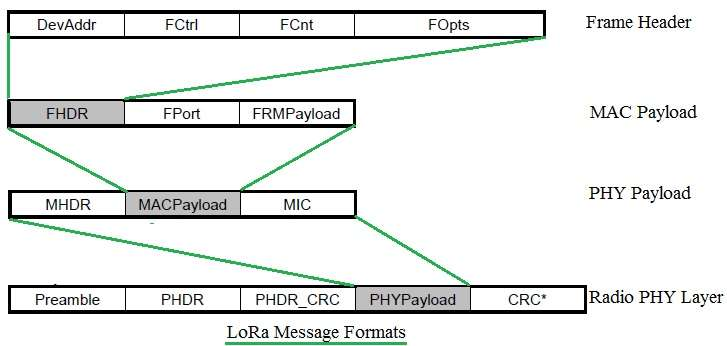
\includegraphics[scale=0.4]{images/LoRa-message-formats}
\caption{Formato de mensaje de protocolo LoRaWAN. Fuente:~\cite{Sornin}}
\label{fig:msg}
\end{figure}
\noindent
Para este proyecto se manipulará el modelo de simulación del protocolo ALOHAnet, con el fin de agregar parámetros de la capa física y de enlace que caracterizan al protocolo LoRa, y así poder imitar el comportamiento de los dispositivos LoRaWAN. Una vez identificados estos parámetros, se incluirán al modelo de simulación, para así tener la capacidad de replicar distribuciones y comportamientos esperados de los dispositivos físicos pero de manera virtual.\\
En cuanto al contenido de cada fragmento de los mensajes enviados por dispositivos LoRa, estos están definidos en las especificaciones técnicas del fabricante, los que son expuestos en la Tabla~\ref{tab:loramsg}~\cite{Sornin}.\\
Los indicadores a usar para el modelo de simulación planeado, son aquellos pertenecientes a la capa RF PHY, a la capa PHY \textit{payload} y la capa MAC \textit{payload}, sin contar tramas de capas superiores, dado que la herramienta de simulación trabaja en sobre la base de eventos, no analizando paquetes como lo haría un ``\textit{sniffer}'' de red, por lo que algunos campos de información contenida en la cabecera del mensaje es omitida dado este antecedente.
\begin{table}[!ht]
\begin{tabular}{|c|l|}
\hline
Campo de mensaje LoRa MAC & Descripción \\\hline
MHDR & Cabecera	MAC, longitud de un octeto\\\hline
MAC \textit{payload}	& Datos de capa superior\\\hline
MIC	Message Integrity Control & longitud de cuatro octetos\\\hline
FHDR  &	Cabecera de tramas de mensaje\\\hline
FPort	& Campo opcional de puerto de conexión\\\hline
FRMpayload	& Campo opcional de \textit{payload} \\&de tramas de mensaje\\\hline
Devaddr	& Dirección de dispositivo\\\hline
FCtrl & Octeto de control de tramas de mensaje\\\hline
FCnt &	Contador de tramas de mensaje,\\& longitud de dos octetos\\\hline
FOpts &	Opciones de trama, usadas para \\&ordenes de transporte\\ & en la capa MAC, longitud de \\&quince octetos\\\hline
\end{tabular}
\caption{Glosario de campos de mensajes LoRa}
\label{tab:loramsg}
\end{table}
En relación al formato del mensaje de LoRaWAN, a continuación se explican cada uno de los campos, y sus funciones dentro de los mensajes de LoRaWAN.\\
\begin{itemize}
\item MAC \textit{Header} (MHDR): Este campo contiene información cómo el tipo de mensaje (MType), donde se pueden tener mensajes como: join request, join accept, confirmed data up, entre otros. Este campo, también contiene la versión del formato de mensaje (Major), donde dependiendo de esta versión, el mensaje podría estar codificado o no. La estructura mencionada en este apartado, puede encontrarse en la Tab~\ref{msg:1}.

\begin{table}[!ht]
\centering
\begin{tabular}{|r|c|c|c|}
\hline
bit & 7..5 & 4..2 & 1..0 \\\hline
MHDR bit & MType & RFU & Major\\\hline
\end{tabular}
\caption{Formato de mensaje, campo cabecera MAC. Fuente:~\cite{Sornin}}
\label{msg:1}
\end{table}

\item MAC \textit{payload}: En este campo se encuentran las tramas de datos a enviar, dentro de este campo se encuentra información como la cabecera de la trama (\textit{Frame Header - FHDR}), seguido de dos campos opcionales, los cuales son \textit{Frame Port -FPort}, y \textit{frame payload- FRMpayload}. Estas campos contenidos en MAC \textit{payload}, serán explicados a continuación.
\begin{itemize}
\item \textit{Frame Header}: Este campo contiene la dirección del dispositivo (nodo) en el campo (DevAddr), un campo de control de trama (FCtrl), adicionalmente posee un contador de trama de mensaje (FCnt) y un campo llamado opciones de trama (FOpts) el cual tiene la función de enviar comandos MAC mediante este campo. Esta estructura puede apreciarse en la Tab~\ref{msg:2}.\\
\begin{itemize}
\item \textit{DevAddr}: Este campo posee la dirección en la red LoRa del dispositivo nodo al cual se le desea enviar la información.
\item \textit{Frame Control}: Aquí es contenida la información sobre el estatus del \gls{adr} (activo o no activo), el estado de llegada del paquete \gls{ack}, el largo del campo FOpts, y dependiendo si es un mensaje de bajada o subida, puede llevar un campo con la información de tramas pendientes (FPending), o tener un campo reservado para usos futuros (RFU) respectivamente.
\item \textit{Frame Counter}: En este campo se almacena el contador de tramas de mensaje, para tener un control sobre cuantos mensajes llegaron del total (en caso de ser paquetes fragmentados), y así pedir retransmisión de datos en caso de necesitarlo.
\item \textit{Frame Options}: Este campo almacena los comandos MAC a enviar, con un máximo de 15 octetos para enviar.
\end{itemize}

\begin{table}[!ht]
\centering
\begin{tabular}{|r|c|c|c|c|}
\hline
Tamaño (bit) & 32 & 8 & 16 & 0..120 \\\hline
FHDR & DevAddr & FCtrl & FCnt & FOpts\\\hline
\end{tabular}
\caption{Formato de mensaje, campo cabecera de trama. Fuente:~\cite{Sornin}}
\label{msg:2}
\end{table}

\item \textit{Frame Port}: Este campo opcional, entrega información del puerto destino, en el dispositivo receptor. En el caso de que el campo FRMpayload esté presente, el campo FpPort también debe estarlo. En el caso de poseer un valor 0 en el campo FPort, el campo FRMpayload, sólo enviará comandos MAC hacia su receptor. Y en el caso de que el valor de FPort, se encuentre entre \num{1}..\SI{223}{\bit}, FRMpayload contendría usos específicos para cada aplicación, mientras que los valores \num{224}..\SI{255}{\bit} en FPort, están reservados para usos futuros.
\item \textit{Frame payload}: En este campo es contenida la información a enviar al destinatario, la que puede variar desde comandos MAC estandarizados de LoRa hacia el receptor, o información específica de cada aplicación a usar con los dispositivos LoRa.
\end{itemize}
\item \textit{Message Integrity Control}: En el campo MIC, se almacena una especie de valor de \textit{hash} que permite comprobar la integridad del mensaje enviado. El valor almacenado en este campo, es calculado sobre todos los campos en el mensaje, y sobre la base del RFC4493.
\end{itemize}
\section{Diferencias entre LoRaWAN y ALOHAnet}
En relación a la diferencia entre LoRaWAN y ALOHAnet, esta radica en que el protocolo LoRa, si bien es implementado sobre la base del sistema ALOHA slotted, LoRaWAN es capaz mediante comandos MAC el colocar en modo reposo a los clientes que no necesiten mandar paquetes, y programar su próxima entrega de información, donde gracias a una sincronización de relojes entre el cliente y la puerta de enlace ( o concentrador LoRa), es posible generar un ahorro de consumo de energía considerable en los nodos, dando así una mayor autonomía a los dispositivos. Cabe destacar, de que ALOHAnet no es un protocolo de comunicación como lo es LoRaWAN, si no un sistema de comunicación inalámbrica para dispositivos, por lo que el tipo de mensajes que se utilicen en ALOHAnet, depende exclusivamente de que protocolo se utiliza sobre este sistema.\\
 En relación a las características de LoRaWAN, este posee una optimización de los usos de los canales de transmisión, ya que a diferencia de LoRa, ALOHA sólo usa una frecuencia para transmitir y otra para recibir información de sus clientes, por lo que si una puerta de enlace, llegaba a alcanzar un determinado número de clientes, las retransmisiones generadas por las colisiones de paquetes en el canal, generarían un colapso de la transmisión/recepción de paquetes denegando cualquier tipo de transmisión entre los actores de la red (Denegación de Servicio por saturación de canal). En cambio LoRaWAN usa la modulación de señal de espectro expandido, esta modulación expande a un mayor tamaño el espectro de la señal necesaria para transmitir un \textit{payload} determinado, esto genera un tipo de blindaje alrededor de la frecuencia base de la señal a interferencias externas de frecuencias angostas. Asimismo, si el receptor conoce la frecuencia base del mensaje enviado, es posible utilizar bandas de frecuencia dentro del espectro expandido, es decir otorga la capacidad de uso de multi-canales, y además mejora la seguridad de la comunicación en contra de intercepciones no deseadas, dado que si el receptor no conoce la frecuencia base, no le será posible filtrar mediante el uso de un filtro correcto de bandas, lo que resultaría en la obtención de sólo el ruido de la señal. Esta técnica de modulación, realiza una concesión de tasa de envío de datos a favor de un mayor alcance de transmisión y viceversa. Este proceso es realizado mediante el uso de canales con un ancho de banda corregido, con el fin de mejorar la comunicación entre nodo/\textit{gateway}, esto permite la optimización de la red a un ancho de banda constante, dado que al usar un espectro de señal expandido, es necesario pasar la señal por un filtro entre bandas o pasa bandas para obtener el contenido de la señal base y poder demodular el contenido sin alteraciones de ruido o interferencias ~\cite{modulation}.

\section{Simulación por eventos discretos}
Una simulación por eventos discretos es un tipo de modelado dinámico de sistemas que se caracteriza por mantener un estado global del sistema, que puede estar distribuido de forma lógica o física y que cambia de forma parcial dada la ocurrencia de un evento en particular. Cualquier estado en el sistema sólo cambia al ocurrir un evento definido previamente, donde uno o varios procesos que tienen por trabajo la ejecución de estos eventos. La ejecución de un evento en un sistema modelado por eventos discretos quita los eventos pendientes para el valor de tiempo actual y agregando unidades de tiempo establecidas en la definición de los parámetros y variables~\cite{simubook}.\\
Con respecto a los eventos, estos se definen como un suceso que realiza modificaciones a las variables de sistema. Todo evento es parte de una entidad u objeto de un sistema simulado, por lo que sólo cambiarán atributos de este, no interviniendo ninguna variable o atributo del resto del sistema~\cite{simubook}.\\
Referente a las entidades, estas se definen como los objetos o actores que en conjunto representan al sistema a simular. El estado global del sistema se conforma por el conjunto de estados de las entidades definidas.\\
En relación con el proyecto de título, se utilizará esta técnica de modelado, dado que se busca modelar el comportamiento físico de los dispositivos LoRa, el cual funciona en base a máquinas de estados o eventos. Este modelado tomará algunas variables como constantes o despreciables con el fin de simplificar el modelo de simulación, es decir, reducir el número de variables con el fin de centrar el foco del modelo de simulación, solamente en el funcionamiento lógico de la capa de enlace y física, junto con agregar parámetros reales existentes en las telecomunicaciones, tales como el porcentaje de pérdida de paquetes, entre otros.\\
Entre las variables a simplificar se encuentran ~\cite{orange}:\\
\begin{itemize}
\item Tasa de codificación (\textit{Code rate}).
\item El ancho de banda.
\item La tasa de envío de bits para cada \gls{sf}.
\item Los rangos de distancia que admite cada \gls{sf} .
\item El desfase de la señal de RF.
\item Tamaño del paquete a enviar.
\item Tiempo en aire del paquete.
\end{itemize}
No obstante, se realizarán mediciones con dispositivos reales, con los mismos valores fijados en los parámetros constantes, y con condiciones semejantes a las simuladas (i.e. atenuación de la señal equivalente a transmitir a una determinada distancia, entre otros.). Y de esta manera, asegurar un margen de error del modelo de simulación. Para determinar este margen de error, se compararán los valores obtenidos en la recepción y envío de paquetes entre los dispositivos reales con un cierto nivel de pérdidas y el modelo de simulación con características homologas. En el caso de que los resultados de las mediciones empíricas tengan sobre un \SI{3}{\percent} de diferencia con los datos del simulador, se realizarán los ajustes pertinentes para que se ajuste a la sensibilidad de error tolerada como válida (a lo más un \SI{3}{\percent}).
\section{Herramientas para simulación de redes}
Dentro de las herramientas de simulación por eventos discretos para redes sobre la base del protocolo ALOHAnet, se encontraron dos herramientas: NS-3 y \OMNET.\\
De estas herramientas se propone la utilización de \OMNET, dado que posee una interfaz gráfica muy amigable para la representación de los datos (representación de comunicación en la red, envío de mensajes, generación de gráficos, etc.), asimismo posee una interfaz de fácil uso para la manipulación de los archivos programables junto a un menú para ajustar variables de la simulación como el retardo de envío de mensajes, etc. Por otra parte, NS-3 si bien es un potente software de simulación, sus últimas versiones han tenido problemas de compilación en algunos módulos, inclusive en la integración del módulo MIXIM e INET al \textit{framework}, módulos que serán necesarios para el desarrollo del módulo de transición de LoRaWAN a IPv6. De la misma forma, se detectó de que NS-3 ha presentado en su última versión, intestabilidad en el desarrollo de simulaciones y problemas de integridad de datos~\cite{bugtrack}. Por estas razones, se ha preferido trabajar con el software \OMNET, el que en su última versión posee un número menor de incidencias sin resolver, en comparación con NS-3~\cite{bugtrack2}. Este antecedente, indica que las mediciones de \OMNET~tendrán mayor nivel de fiabilidad, que un programa que posee un mayor número de errores sin resolver.

\end{justify}